\documentclass[11pt,a4paper]{report}
\usepackage[utf8]{inputenc}
\usepackage[T1]{fontenc}
\usepackage{microtype}
\usepackage[dvips]{graphicx}
\usepackage{xcolor}
\usepackage{times}
\usepackage{ragged2e}
\usepackage{titlesec}
\usepackage{wrapfig,subfigure,setspace,verbatim,cite,url,graphicx,float}
\usepackage{algorithmic,amsfonts,amssymb,amsmath,calc,calrsfs,cleveref}
\usepackage[justification=centering]{caption}

\usepackage[
breaklinks=true,colorlinks=true,
%linkcolor=blue,urlcolor=blue,citecolor=blue,% PDF VIEW
linkcolor=black,urlcolor=black,citecolor=black,% PRINT
bookmarks=true,bookmarksopenlevel=2]{hyperref}

\usepackage{geometry}
% PDF VIEW
\geometry{total={210mm,297mm},
left=25mm,right=25mm,%
bindingoffset=0mm, top=25mm,bottom=25mm}
%PRINT
\geometry{total={210mm,297mm},
left=20mm,right=20mm,
bindingoffset=0mm, top=15mm,bottom=35mm}

\linespread{1.5}

\titleformat{\chapter}
{\normalfont\LARGE\bfseries}{\thechapter.}{1em}{}

%%%---%%%---%%%---%%%---%%%---%%%---%%%---%%%---%%%---%%%---%%%---%%%---%%%

\begin{document}

%%%---%%%---%%%---%%%---%%%---%%%---%%%---%%%---%%%---%%%---%%%---%%%---%%%
%   TITLEPAGE
%
%   due to variety of titlepage schemes it is probably better to make titlepage manually
%
%%%---%%%---%%%---%%%---%%%---%%%---%%%---%%%---%%%---%%%---%%%---%%%---%%%
\thispagestyle{empty}

{%%%
\sffamily
\centering

{\Large 
Parallelization of Push-based System for Molecular Simulation Data Analysis with GPU
}

\vspace{1.5cm}

{
by
}
\vspace{.5cm}

{ 
Iliiazbek Akhmedov
}

\vspace{3.5cm}

A thesis submitted in partial fulfillment

of the requirements for the degree of

Master of Science in Computer Science

Department of Computer Science and Engineering

College of Engineering

University of South Florida

\vspace{3.5cm}
Major Professor:  Yicheng Tu, Ph.D.
\vspace{\fill}


\vspace{.5cm}
Date of Approval:

N/A
\vspace{\fill}

Copyright \textcopyright\space 2016, Iliiazbek Akhmedov

%%%
}%%%

\clearpage

\newgeometry{left=20mm,right=20mm,top=35mm,bottom=35mm}

\pagestyle{plain}
\centering

\textbf{DEDICATION}
\vspace{0.5cm}

\begin{flushleft}
\hspace{3em} I dedicate my thesis work to my family who have always been supporting me throughout my life. I also dedicate it to my closest friends who have shared my passion and encouraged me to explore and try my ideas in life.
\end{flushleft}

\clearpage

\pagestyle{plain}
\centering
\textbf{ACKNOWLEDGMENTS}
\vspace{0.5cm}

\begin{flushleft}
\hspace{3em} I would like to thank my major professor throughout my master thesis Dr. Yicheng Tu for his guidance and knowledge that I received through all the time I worked with him. I really appreciate his contribution and very happy that I got a chance to work with him. I as well want to thank the committee members for their support and encouragement.
\end{flushleft}

\clearpage
\restoregeometry

\tableofcontents

\clearpage

\begin{abstract}
\justify
\hspace{3em} Modern simulation systems generate big amount of data, which consequently has to be analyzed in a timely fashion. Traditional database management systems follow principle of pulling the needed data, processing it, and then returning the results. This approach is then optimized by means of caching, storing in different structures, or doing some sacrifices on precision of the results to make it faster. When it comes to the point of doing various queries that require analysis  of the whole data,  this design has the following disadvantages: considerable overhead on random I/O while reading from the simulation output files and low throughput of the data that consequently results in long latency, and, if there was any indexing to optimize selections, overhead of storing those becomes too big, too. 

There is a new approach to this problem presented in the previous paper -- Push-based System for Molecular Simulation Data Analysis for processing network of queries proposed in the previous paper and its primary steps are: i) it uses traditional scan-based I/O framework to load the data from files to the main memory and then ii) the data is pushed through a network of queries which consequently filter the data and collect all the needed information which increases efficiency and data throughput. It has a considerable advantage in analysis of molecular simulation data, because it normally involves all the data sets to be processed by the queries.

In this paper, we propose improved version of Push-based System for Molecular Simulation Data Analysis. Its major difference with the previous design is usage of GPU for the actual processing part of the data flow. Using the same scan-based I/O framework the data is pushed through the network of queries which are processed by GPU, and due to the nature of science simulation data, this gives a big advantage for processing it faster and easier. In the old approach there were some custom data structures such as quad-tree for calculation of histograms to make the processing faster and those involved loss of data and some expectations from the data nature, too. In the new approach due to high performance of GPU processing and its nature, custom data structures were not even needed much though it didn't bear any loss in precision and performance.
\end{abstract}

%%%---%%%---%%%---%%%---%%%---%%%---%%%---%%%---%%%---%%%---%%%---%%%---%%%
%%%---%%%---%%%---%%%---%%%---%%%---%%%---%%%---%%%---%%%---%%%---%%%---%%%

\chapter{Introduction}

\justify
In various sciences simulation systems take big place and often times they may be the clue for results. One of such sciences, which is primarily related to this paper, is physics. In this case, from computer engineering point of view, simulations have the following flow:

\vspace{5mm}

\begin{enumerate}
	\item initial physical properties are given to simulation software as arguments which are interpreted and provided in a language defined by the simulation software
	\item then it runs for given amount of time that can generally last from milliseconds to months or even more
	\item finally, the file generated during the simulation is analyzed to extract useful information
\end{enumerate}

\vspace{3mm}
The purpose of this paper is primarily focused on the third step, which basically involves the entire simulation data to be processed by the analysis software.

Big data processing is becoming one of the key issues with the amount of data being generated by modern systems. Eventually, this data is required to be processed on the fly, thus, analysis software should be able to handle massive data in a very short period of time. When working with huge volume of data, there are non-trivial issues arise. For example, it can take days and weeks to analyze big enough data sets, because the data cannot be simply loaded into memory, since it can get up to terabytes, thus, it has extra overhead because of traditional random access disk I/O framework to read from disk chunks by chunks. Besides it, analysis of the data can get even more complicated, since going through certain parts of the data once would not be enough, which leads to low throughput and efficiency of loaded data. One such example, the data analysis approach has polynomial complexity just for reading the data in order to come up with result, and since the data can't simply be saved in memory, it raises the overhead of disk I/O, too. Pull-based architectures in data processing engines are inefficient, since having a set of specific queries, in order to compute them all, it is needed to fetch data, filter it, and apply needed formulas. It is inefficient, since for every query the same chunk of data needs to be pulled into the memory at least the number of queries times or more in case of more complex queries.

As it has already been mentioned in the previous paper \cite{mainPaper}, one of the modern issues of analyzing massive data on the fly is social networks. "In order for a system to be able to perform analytical examination of the data produced in such streaming media, the system should have the capability of fast data access. The reason, the millions of data records (tweets) produced every second. Moreover, these tweets may have different geographical origin, introducing different languages and forms and often times containing unsolicited messages, errors,
malicious content, etc. Therefore, some low level data uniformity
and cleaning on top of the data access and management issues should
be considered and possibly incorporated in the process of analytical
investigation in order to achieve relevant result. "\cite{mainPaper, nature_bigdata08,nature_bigdata12,science_social10,jcs_twitter11}

The primary focus and problem in this paper is scientific data analysis. Particles simulation is one of the most popular methods of analyzing certain chemical reactions, physical processes, or other behavior of different materials.
Molecular simulations (Molecular Dynamics) are applied in different fields and represent a method of analyzing physical movements of particles, atoms, and molecules in a fixed space with a given period of time, apparently with a possibility of giving initial state for each item that is involved in the process and can affect the system. This system is an N-body simulation. The number of atoms in simulations vary in hundred of thousands, particularly, we may observe two simulation systems of a collagen fiber structure and dipalmitoylphosphatidylcholine (DPPC) bi-layer lipid system consisting of 890,000 and 402,400 atoms respectively on Figure \ref{fg:collagen_dipal}. Simulation data represents number of records of physical properties such as mass, charge, velocity, coordinates, and forces for each item aggregated as frames, where each frame represents a snapshot of time, placed with a fixed time interval which may also vary depending on the simulation itself and simulation precision requirement. "Quantities measured during the simulations are analyzed to test the theoretical
model~\cite{Frenkel:api01,Landau:cup05}. In short, the MS is proven
and powerful tool for understanding the inner-workings of a
biological system, by supplying a model description of the
biophysical and biochemical processes that are being unfold at a
nanoscopic scale." \cite{mainPaper}

Scientist gives the properties to simulation software (for example, Gromacs), runs the simulations, and finally get the output file. The output file must then be analyzed to produce certain results which may help him come up with certain consensus on original theoretical model that resulted in the molecular simulation system\cite{Frenkel:api01}. Gromacs is simulation software tool that helps scientist to run the actual simulation. It is a molecular dynamics package primarily designed for biomolecular systems such as proteins and lipids. \cite{Gromacs-online}. Besides the fact that it helps to generate the output files for the simulations, apparently it also helps to analyze the data itself, but the original problem is that it is not as optimized as it can be in order to analyze the data. Gromacs follows approach of pull-based design, which means that for any given query (e.g. total mass or total charge, which are very similar type of 1-body queries without sophisticated selection) it will pull data separately and generate addition overhead wasting disk read I/O in order to come up with the result just for a single query. As it has been proposed in the previous paper, in order to remedy such issues, the push-based design does exactly the opposite, where instead of loading the data on demand for each query, the queries are batched into a network, then the entire dataset is loaded chunk by chunk pushing it through the network which has its internal relationships and dependencies amonth the queries. In this case, since scientific simulation data is run once with specific physical properties, it is never modified, thus, on continuation, it will only append, which means that the processing can also be run on appended frames. \cite{mainPaper}
This type of approach has already been revised by other systems \cite {DataPath,Volcano,Qpipe} as of reusing loaded data through queries produced \cite {Candea,PredictablePerformance,CooperativeScans}.

In this paper, we are incorporating parallelization into the processing part of the proposed design by means of CUDA programming language for GPU. Since storage of the simulation data is very expensive, it might come to the point of analyzing the data on the fly (meaning running the simulation and analyzing it at the same time in a streaming manner), which leads to a problem of optimizing the processing part of the design proposed in the previous paper, because time spent on generating data should be tried to conceal the time spent on the processing part by means of overlapping or simply running it in a quick manner.

\begin{figure}
 \centerline{ \includegraphics[width=0.5\columnwidth]{images/sample_snapshot_of_simulation.eps} }
 \caption{ Snapshots of two MS systems: a collagen fiber structure with 890,000 atoms (top) and a dipalmitoylphosphatidylcholine (DPPC) bi-layer lipid system with 402,400 atoms (bottom) \cite{mainArticle}}
 \label{fg:collagen_dipal}
\end{figure}


\section{Problem Statement}
Simulation software systems, in general, follow the same methodology of running and storing simulation data. The simulation software system examples are: Gromacs \cite{GROMACS4}, VMD\cite{VMD}, MDAnalysis~\cite{MDAnalysis}, Wordom~\cite{wordom}, MD-TRACKS~\cite{MDtracks}, SimulaidOne~\cite{Simulaid}, Charmm~\cite{CHARMM}. In the type of simulations brought up as examples above, the flow of the data is the following. Once the simulation is run, the output files are contained as trajectory files with descriptors (they contain information about space dimensions, number of atoms and frames, etc.) that can be easily transposed into simple flat files containing the physical properties atom by atom, frame by frame, which are consequently read and processed by the proposed push-based system. Since we have certain amount of queries needed to be run on given simulation data, generating high I/O traffic followed by design of pull-based system is not considerable. The approach proposed in the previous paper is very good in terms of performance in comparison with the original pull-based system\cite{mainPaper}. The problem is still that some of the queries processed by those means are still improvable, especially taking into consideration the fact that in the used previous works for calculation of 2-body functions, which take the biggest time for processing~\cite{ytu:icde09, EDBT12}, we might have some error bounds, which might be unacceptable for certain simulation analysis where sacrifice on loss of data is unbearable. Besides it, although we might have huge performance boost on specific data structure as density map, we still have certain expectation from data nature (such as its uniformity), thus, it makes sense to have desire to simplify the processing and still having pure computation based on any values, considering that the queries should be available to be pre-programmed by user in a separate module of the code.

\begin{figure}
 \centerline{ \includegraphics[width=0.5\columnwidth]{images/speedup838K-pomalo-za-4.eps} }
 \caption{ Speed up over different levels of atom selection for 838,400 atoms \cite{mainPaper}}
 \label{fg:sample_estimation_old_paper}
\end{figure}

\section{Our approach with improvement}

Reading the data from files is a huge overhead, thus, speedup of push-based system in general is significant over pull-based system in our given case. 
It's been demonstrated in the previous paper with different amount of atoms, frames, and workloads. Since we have to load the data every time there is a different query versus push-based system loads a chunk of data once, it is quite noticeable how the framework contributes to efficiency of analysis of simulation data. You can observe some estimation samples in Figure \ref{fg:sample_estimation_old_paper}. Even though the memory loading and pushing steps are the key features of the proposed design, nevertheless, having general knowledge about the network of queries, in this paper, we will try to focus on optimizing the actual execution of them.

Some of the queries may be very slow due to their nature on a sequential type of computation,  especially, 2-body functions. Since the nature of the data that comes with simulation is basically physical properties of atoms, there is a lot of computation that involves independent primitive mathematical operations, which makes it a perfect problem for parallelism.

Although the original idea of push-based system for molecular simulation data analysis was focused on optimizing throughput and usage of loaded data, there were some extra approaches specifically for 2-body functions. For example, Density Map for Spacial Distance Histogram was used in order to avoid additional memory allocation and latency reduction with proven error bounds. SDH is a quite intensive and computational problem, especially with increasing amount of atoms. 

We believe that having this nature of computational problems, the proposed GPU improved version of push-based system will significantly change in terms of performance by incorporating parallelism with CUDA.

%%%%%%%%%%%%%%%%%%%%%%%%%%%%%%%%%%%
%%%%%%%%%%%%%%%%%%%%%%%%%%%%%%%%%%%
\begin{figure}
\centering
\centerline{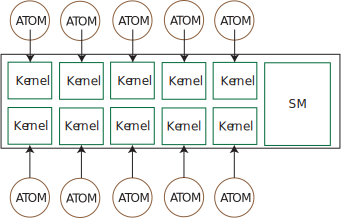
\includegraphics[width=0.5\columnwidth]{images/kernelatom.eps}}
\caption{ Example of atom mapping with kernels}
 \label{fg:kernelatom}


\end{figure}
%%%%%%%%%%%%%%%%%%%%%%%%%%%%%%%%%%%
%%%%%%%%%%%%%%%%%%%%%%%%%%%%%%%%%%%

\section{Contribution and roadmap of the paper} 
The proposed improved version of push-based system for molecular simulation data analysis, we believe, gives an opportunity for scientists to run their analysis even faster now. Taking an advantage of GPU devices nature and incorporating parallelism and streaming for different types of queries, we have come up with a good speed up over sequential processing, which already had a good speed up in terms of performance in comparison with original pull-based approach. Since in this paper we don't expect certain form of data, we have come up with a tool that generates mock data for any number of atoms and frames, which can be used for performance tests that were done consequently, too. This mock data has exactly the same information that would come with Gromacs simulation files, and it has exactly the same format as in the previous paper \cite{mainPaper} right before loading it to memory. This improved version has been developed on Amazon Elastic GPU \cite{amazonGPU} nodes that consequently can be replicated and scaled up becoming more of a streaming distributed processing engine (which can be very effective on costs, since it is always easy to scale them up, shut them down and spin them back up), as well as on a simple desktop computer with a GPU device.
In general, major contribution of this paper is the framework of push-based system with an incorporated parallelism based on CUDA programming language. Besides it, there was developed a tool which generates mockup data of the same format as of the real MS simulations and represent a python script with arguments given as number of frames and atoms.

The structure of the framework which will be described later is developed in such a way that one can easily add new queries based on their complexity or modify existing ones adding appropriate selections and filters.


%%%%%%%%%%%%%%%%%%%%%%%%%%%%%%%%%%%%%%%%%%%%%%%%%%%%%%%%%%%%%%%%%%%%%%%%%%%%%%%

\chapter{Related Work}\label{sc:relatedwork}

Push-based system for MS data analysis is primarily proposing an idea of pushing chunks of data through a network of queries. Essentially, this has also been proposed, as mentioned already, by other frameworks \cite{DataPath,Volcano,Qpipe}. In other words, the major point is to use common data loaded into memory for execution of concurrent queries, which is supposed to eliminate I/O overhead predominantly. The architecture and explanation of DSMS (Data Stream Management System) versus DBMS is well explained in one of the lectures of Morgan and Claypool \cite{DataStreamManagement}. It is very important to capture the differences and specialties of DSMS in network architecture, stream models and windows, scheduling, load balancing, approximation, data expiration, etc, because of the fact that data flow design is the key that required all of those changes to common designs.

Since dealing with data is very delicate in this kind of engines, there are couple of features and requirements that this architecture is applicable to, in order to avoid inappropriate understanding or application of this approach in systems that were covered in the lectures\cite{DataStreamManagement}. The data is volatile and not persistent anymore because of obvious sizes of data.  Since we are pulling the data as little times as possible taking into consideration that MS data is only appended and not modified, the access is sequential rather than random. There are concepts of framing and windowing, and memory is limited in streaming engine, while in DBMS secondary storage is considered to be unlimited. Obviously, because of all of these features or requirements to data, the streaming engine frameworks have some limitations like going back into the history of data, since it is volatile. In fact, this has also been tried by Borealis Streaming Engine \cite{borealis}. On top of the fact that it is a streaming engine, as it was built based on Medusa\cite{medusa} and Aurora\cite{aurora}, it proposes distributed processing at this point having some features to handle errors and look back in the history. In our case, it is primarily a single data source, since it is based on the simulation, though in the future the simulation software systems might introduce distributed computing, too. It is also important to mention such projects as PeriScope\cite{PeriScope}, SciDB\cite{SciDB}, and other\cite{SDSS_SIGMOD02,QBISM_ICDE94}, since they target scientific data, which is a lot more different, than usual industry customer oriented data.

This version of Push-based System of MS data analysis is primarily about taking an advantage of GPU processing of the data. Hadoop is a well-known and well-used framework by many companies nowadays\cite{hadoop}. Its purpose is an ability to store and serve large scale data across clusters in a timely fashion. Since usage of GPU of massive data (not only related to graphics processing) is a relatively new concept, there is also an improved version of Hadoop MapReduce Framework with GPU\cite{hadoopgpu}. Having an ability to scale it up in a distributed computing environment is probably one of the best approaches, but again it might be a bigger overhead in terms of costs, since keeping all nodes up and still being able to solve specific problem sets with hardware stack of a lower capacity raise a will to explore more. Having a specific software for simulation like Gromacs, apparently there is also a possibility of taking an advantage of GPUs. For example, Gromacs allows to optimize simulation and query tools by adding configurations based on GPU device located on the processing computer. Unfortunately, even with this feature, Gromacs doesn't follow push-based approach which means that improvement with GPU with pull data per query makes it negligible.

Gromacs generate output files with physical properties description for each atom in each frame. Modern CPUs do great job in terms of caching and computing, but obviously in this particular problem massive monolithic computation is needed, thus, GPU devices are perfect candidates for such a problem following SIMD type of computation. To be more exact, for example, a single kernel in a GPU device could be dedicated to a single atom (this relationship might change depending on the query, but this is to understand the scale and relationship of multiprocessors), and since we have scientific data of MS, the data is appended, which means that we will only move forward and not take an advantage of caching on chunks high level (though we might take an advantage of GPU caching features particularly in processing phase) having multiple workloads per chunk. Just to make it more clear, workloads in this particular case represent transactions based on number of clients. For example, if we were to serve it all in a streaming fashion, 100 clients might demand concurrent queries with different slight selection properties and expect their results, each workload might be dedicated to each client if not aggregated. Thus, the performance of GPU is certainly increasing based on workload too, which might benefit considerably.


\section{Network of Queries}\label{sc:querynetwork}
Having generated big amount of data in large files, now scientists need to get useful information out of it by means of analysis utilities. Often times, the queries that need to be run over the data look like selection and some kind of accumulation, if it is not more complicated. To be more exact, in this section we will try to summarize common set of queries we will be improving. 

In previous work, there has already been developed a network of queries widely used by scientists for MS systems. In Table~\ref{tb:queries} you may observe the common set of queries that has been developed. Basically, these are the queries that need to be improved with our new approach of parallelism. Just to mention, $n$, $r_i$, $m_i$, $c_i$ and $q_i$ denote number of particles, coordinates (vector form), mass, charge, and number of electrons of a particle $i$.


\begin{table}[h]
\resizebox{\columnwidth}{!}{\begin{minipage}{\columnwidth}
\renewcommand*{\arraystretch}{1.5}
\tabcolsep=0.12cm
\begin{tabular}{|c| c|}
\hline %inserts horizontal line
Function Name & Equation/Description \\[0.5ex] \hline
Moment of Inertia & $\begin{array} {lcl} I & = & \sum\limits_{i=1}^n m_ir_i \end{array}$ \\[0.5ex]
\hline
Moment of Inertia on z axis & $\begin{array} {lcl} I_z & = & \sum\limits_{i=1}^n m_ir_{zi} \end{array}$ \\[0.5ex]
\hline
Sum of masses & $\begin{array} {lcl} M & = & \sum\limits_{i=1}^n m_i \end{array}$ \\[0.5ex]
\hline
Center of mass & $\begin{array} {lcl} CoM & = & \frac{I}{M} \end{array}$ \\[0.5ex]
\hline
Radius of Gyration & $\begin{array} {lcl} RG & = & \sqrt{\frac{I_z}{M}} \end{array}$ \\[0.5ex]
\hline
Dipole Moment& $\begin{array} {lcl} D & = & \sum\limits_{i=1}^n q_ir_i \end{array}$ \\[0.5ex]
\hline
Dipole Histogram & $\begin{array} {lcl} D_z & = & \sum\limits_{i=1}^n \frac{D}{z} \end{array}$ \\[0.5ex]
\hline
Electron Density & $\begin{array} {lcl} ED & = & \frac{\sum\limits_{i=1}^n (e_i-q_i)}{dz \cdot x \cdot y} \end{array}$ \\[0.5ex]
\hline
Heat Capacity & $\begin{array} {lcl} HC & = & \frac{3000 \cdot \sqrt{T} \cdot boltz}{2 \cdot \sqrt{T}-n \cdot df \cdot VarT} \end{array}$ \\[0.5ex]
\hline
Isothermal Compressibility & $\begin{array} {lcl} I & = & \frac{VarV}{V_{avg} \cdot boltz \cdot T \cdot PresFac} \end{array}$ \\[0.5ex]
\hline
Mean Square Displacement& $\begin{array} {lcl} msd & = & \langle (r_{t+\Delta_t}-r_t)^2 \rangle \end{array}$ \\[0.5ex]
\hline
Diffusion Constant & $\begin{array} {lcl} D_t & = & \frac{6 \cdot msd(t)}{t} \end{array}$ \\[0.5ex]
\hline Velocity Autocorrelation & $\begin{array} {lcl} V_{acor} & =&
\langle (V_{t+\Delta_t}\cdot V_t) \rangle \end{array}$ \\[0.5ex]
\hline
Force Autocorrelation & $\begin{array} {lcl} F_{acor} & = & \langle (F_{t+\Delta_t} \cdot F_t) \rangle \end{array}$ \\[0.5ex]
\hline
Density Function & Histogram of atom counts \\[0.5ex]
\hline
SDH & Histogram of all distances \\[0.5ex]
\hline
RDF & $\begin{array} {lcl} rdf(r) & = & \frac{SDH(r)}{4 \cdot \pi \cdot r^2 \cdot \sigma_r \cdot \rho} \end{array}$ \\[0.5ex]
\hline
\end{tabular}
\caption[Table caption text]{Popular analytical queries in MS\cite{mainPaper} }
\label{tb:queries}
\end{minipage} }
\end{table}

In general, with the given queries we have divided them into two categories: one body functions and multiple body functions. The first ones apparently have linear complexity of $O(n)$, while the other ones have bigger complexity. 

\emph{\textbf{One body functions}} such as sum of masses, center of mass, or simple counting with selection  are of a complexity $O(n)$, thus, in order to get the results for them going through every atom (essentially over the entire data) only once is enough, and taking into consideration the fact that we are going with push-based system, it is done at the same time for all of them. 

\emph{\textbf{Multiple body functions}} such as SDH and RDF (Spacial Distance Histogram and Radial Distribution function) require computation of distances pairwise across all the particles. This is generally combination of two across N data: 	$C\binom{N}{2}$. These are the most expensive queries, thus, it is important to focus on their implementation taking advantage of GPU nature and its processing power. SDH is a very expensive computation, and we have used some of the existing work of ours\cite{sdhgpu} to incorporate in this design.

The might be some dependencies and preliminary computation possibilities. For example, some queries need total mass, and we could compute it before we push it further, but this can be easily done by user based on the complexity and dependency. It is explained in more details in further sections.


\bibliographystyle{unsrt}
\bibliography{references.bib}

\end{document}

